\chapter{Krachten op het schip}
\vspace{-120px}
\question{1}{Hoe zorg je ervoor dat je boot sneller oploeft?}
\answerTextFour{Door meer mensen aan de lijkant te zetten (lage kant)}{Door meer mensen aan de loefkant te zetten (hoge kant)}{Door je zwaard op te doen}{Door je grootzeil te vieren}


\question{2}{Wat is er fout aan het zeil in het figuur hiernaast?}
	\vspace{-20px}
\begin{figure}[H]		
	\begin{minipage}[]{0.70\textwidth}
		\begin{enumerate}[topsep=0pt, label=\Alph*.]
			\item Het zeil staat te strak
			\item Het zeil staat te los
			\item Het zeil is slecht gehesen
			\item Het zeil is kapot
		\end{enumerate}
	\end{minipage}
	\begin{minipage}[]{0.29\textwidth}
		\begin{figure}[H]
			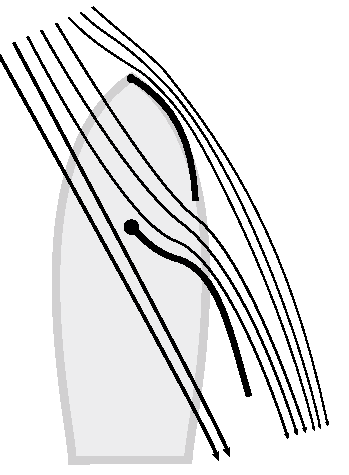
\includegraphics[width=0.60\textwidth,right]{Hoofdstukken/Krachten/pdf/trimmen_los.pdf}
		\end{figure}
	\end{minipage}
	\vspace{-20px}
\end{figure}



\question{3}{Je vaart halve wind en wil snel oploeven, wat doe je?}
\answerTextFour{Beide zeilen vieren}{Je fok vieren en grootzeil aantrekken}{Je grootzeil vieren en fok aantrekken }{Beide zeilen aantrekken}

\question{4}{Hoe controleer je of je grootzeil goed staat?}
\answerTextFour{Door je zeil te laten vieren}{Door deze te laten vieren tot hij tegenbolt en daarna een klein beetje aan te trekken}{Door een beetje af te vallen}{Door naar je zeillatjes te kijken}

\question{5}{Wat gebeurt er als het schip meer naar loef helt?}
\answerTextFour{De loefgierigheid neemt toe}{Het oprichtend koppel neemt af}{De loefgierigheid neemt af}{De zeilkracht neemt af}

\question{6}{Welke vorm van stabiliteit heeft een scherp schip met een kiel?}
\answerTextFour{Vormstabiel}{Natuurlijk stabiel}{Kielstabiel}{Gewichtsstabiel}

\question{7}{Wat is het lateraalpunt?}
\answerTextFour{Het punt waar alle laterale krachten van het schip op werkt}{Het punt waar alle voortstuwende kracht van het schip op werkt}{Het punt waar alle oprichtende krachten van het schip op werken}{Het punt waar alle drijfkracht van het schip op werkt}

\question{8}{Welke onderdeel is een driftbeperkend middel?}
\answerTextFour{Zwaard}{Roer}{Onderwaterschip}{Alle bovenstaande onderdelen}